\documentclass[hyperref]{ctexart}
\usepackage[left=2.50cm, right=2.50cm, top=2.50cm, bottom=2.50cm]{geometry} %页边距
\usepackage{helvet}
\usepackage{amsmath, amsfonts, amssymb} % 数学公式、符号
\usepackage[english]{babel}
\usepackage{graphicx}   % 图片
\usepackage{url}        % 超链接
\usepackage{bm} 
\usepackage{graphicx}        % 加粗方程字体
\usepackage{multirow}
\usepackage{booktabs}
\usepackage{algorithm}
\usepackage{algorithmic}
\renewcommand{\algorithmicrequire}{ \textbf{Input:}}       
\renewcommand{\algorithmicensure}{ \textbf{Initialize:}} 
\renewcommand{\algorithmicreturn}{ \textbf{Output:}}     
%算法格式
\usepackage{fancyhdr} %设置页眉、页脚
\pagestyle{fancy}
\lhead{CN}
\chead{{\Large \textbf{说\hspace{1em}明\hspace{1em}书}}}
\rhead{\thepage/3}
\cfoot{3}
\usepackage{hyperref} %bookmarks
\hypersetup{colorlinks, bookmarks, unicode} %unicode
\usepackage{multicol}
\usepackage{indentfirst} %%缩进

%opening
\begin{document}
	\thispagestyle{empty}
	\clearpage

\begin{flushleft}
	\textbf{{\Large(19) 中华人民共和国国家知识产权局}}
\end{flushleft}
\begin{center}
\textbf{{\LARGE (12)发明专利申请}}
\end{center}



\begin{flushright}
	\textbf{(10)申请公布号}

	\textbf{(43)申请公布日}
	\rule[18pt]{17.3cm}{0.1em}
\end{flushright}
\begin{flushleft}
	\textbf{(21)申请号 }

\textbf{(22)申请日}

\textbf{(71)申请人}\quad  xxxx大学

\hspace{2.5em}\textbf{地址} \quad\hspace{0.5em}330013\quad xxxxxx号


\textbf{(72)发明人}\quad xxx\quad xxx\quad xxx 

\textbf{(51)int.CI.}

\quad\quad\textit{\textbf{B60P 1/02}(2006.01)}
\end{flushleft}
\begin{flushright}
	权力要求书1页  说明书3页  附图2页
	\rule[16pt]{17.3cm}{0.1em}
\end{flushright}
\begin{multicols}{2}
\begin{flushleft}
	\textbf{(54)发明名称}
\end{flushleft}
{\large  xxxxxxxxxxx}\\
\textbf{(57)摘要}

{\large 猫,属于猫科动物,分家猫、野猫,是全世界家庭中较为广泛的宠物。家猫的祖先据推测是古埃及的沙漠猫,波斯的波斯猫,已经被人类驯化了3500年(但未像狗一样完全地被驯化)。一般的猫:头圆、颜面部短,前肢五指,后肢四趾,趾端具锐利而弯曲的爪,爪能伸缩。夜行性。以伏击的方式猎捕其它动物,大多能攀援上树。猫的趾底有脂肪质肉垫,以免在行走时发出声响,捕猎时也不会惊跑鼠。行进时爪子处于收缩状态,防止爪被磨钝,在捕鼠和攀岩时会伸出来。}
\newline
\newline\\
\newline\\
\newline
\begin{figure}[H]
	\begin{center}
		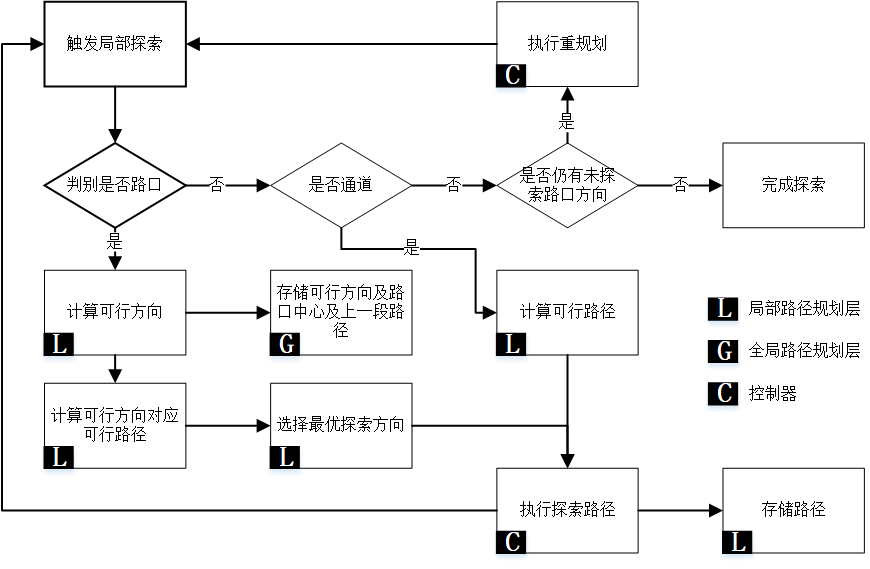
\includegraphics[width=0.7\linewidth]{graph/structure.png}
	\end{center}
	\begin{center}
		 \qquad \qquad 图1
	\end{center}
	\label{fig:tstmp20211203103404}
\end{figure}

	\end{multicols}
\thispagestyle{empty}
\clearpage

\end{document}